
\documentclass{tufte-handout}

%\geometry{showframe}% for debugging purposes -- displays the margins

\usepackage{amsmath}

% Set up the images/graphics package
\usepackage{graphicx}
\setkeys{Gin}{width=\linewidth,totalheight=\textheight,keepaspectratio}
\graphicspath{{graphics/}}

\title{Glycolysis}
\author{}
\date{}  % if the \date{} command is left out, the current date will be used

% The following package makes prettier tables.  We're all about the bling!
\usepackage{booktabs}

% The units package provides nice, non-stacked fractions and better spacing
% for units.
\usepackage{units}

% The fancyvrb package lets us customize the formatting of verbatim
% environments.  We use a slightly smaller font.
\usepackage{fancyvrb}
\fvset{fontsize=\normalsize}

% Small sections of multiple columns
\usepackage{multicol}

% Provides paragraphs of dummy text
\usepackage{lipsum}

% These commands are used to pretty-print LaTeX commands
\newcommand{\doccmd}[1]{\texttt{\textbackslash#1}}% command name -- adds backslash automatically
\newcommand{\docopt}[1]{\ensuremath{\langle}\textrm{\textit{#1}}\ensuremath{\rangle}}% optional command argument
\newcommand{\docarg}[1]{\textrm{\textit{#1}}}% (required) command argument
\newenvironment{docspec}{\begin{quote}\noindent}{\end{quote}}% command specification environment
\newcommand{\docenv}[1]{\textsf{#1}}% environment name
\newcommand{\docpkg}[1]{\texttt{#1}}% package name
\newcommand{\doccls}[1]{\texttt{#1}}% document class name
\newcommand{\docclsopt}[1]{\texttt{#1}}% document class option name

\begin{document}

\maketitle% this prints the handout title, author, and date

\begin{abstract}
\noindent This lecture will cover glycolysis, the backbone of metabolism.  This pathway is especially important because it is the intersection of several pathways of carbohydrate metabolism (gluconeogenesis, glycogenesis, glycogenolysis and the TCA cycle) as well as both the source and result of amino acid synthesis and degradation.  An understanding of how glucose flows through glycolysis is also important for understanding how other monosaccharides such as fructose and galactose are metabolized.  We will cover the regulation of glycolysis by energy status, key metabolites and hormones.  While most of the reactions are listed here, focus on the key steps of control and how they are regulated.  
\end{abstract}

\tableofcontents
\pagebreak
\section{Learning Objectives}

\begin{itemize}
\item Define the role relative locations of of glycolysis, gluconeogenesis, the TCA cycle as nodes of carbohydrate metabolism.
\item Assess the enzymatic differences and tissue distributions of glucokinase vs hexokinase and explain why this is important.
\item Calculate how much ATP is produced from glycolysis, and the relative efficiency of aerobic vs non-aerobic glycolysis.
\item Summarize the key points of regulation of glycolysis and what metabolites and hormones regulate these enzymes.
\item Evaluate the differences between how muscle and liver glycolysis are regulated.  Assess why this is relevant for the functions of these tissues.
\item Describe the potential fates of pyruvate, and what enzyme activities dictate the next steps in its metabolism.  Given a particular cellular state, you should be able to predict which pathway pyruvate enters.
\item Discriminate how non-glucose carbohydrates such as galactose and fructose enter glycolysis, and how their point of entry affects how they are regulated.
\item Predict the effects of specific inborn errors in glucose, galactose and fructose metabolism based on the location of the affected  enzyme in the relevant pathways.  Consider dietary treatments that may be useful in these individuals.

\end{itemize}

\section{Key Concepts, Abbreviations and Vocabulary}

\begin{description}
	\item[Concepts:] Glucose transport, glucose oxidation, negative feedback, feed-forward regulation, inborn errors of metabolism.  
	\item[Key Enzymes and Proteins:] AMPK, PKA, GLUT2, GLUT4, GLUT5, Hexokinase (HK), Glucokinase (GK), Glucose-6-Phosphatase (G6Pase), Phosphofructokinase 1 and 2 (PFK1/2), Pyruvate Kinase (PK), Alanine Aminotransferase (ALT), Pyruvate Dehydrogenase (PDH\sidenote{covered in more detail next lecture.}).  You should be able to locate the relative location of these enzymes in glycolysis, and how they are regulated by metabolites and hormones.
	\item[Important Metabolites:] Glucose-6-Phosphate (G6P), Fructose-1,6-bisphosphate (F16bP), Fructose-2,6-bisphosphate (F26bP), ATP, AMP, Alanine.

\end{description}

\pagebreak

\section{Glycolysis converts glucose to pyruvate}

Glycolysis is the process by which glucose is catabolized to pyruvate.  The conversion of glucose to pyruvate can be the first step to full oxidation of glucose to carbon dioxide, or it can end with pyruvate being released as lactate.  This is the backbone of metabolism, as most carboydrate, amino acid and lipid metabolic pathways involve glycolysis in one way or another.  For a refresher on glycolysis, we recommend the textbooks on reserve at the Shapiro library \citep{Berg2013,Ferrier2017}\sidenote{The relevant chapter of Berg is also available free here: \url{https://www.ncbi.nlm.nih.gov/books/NBK22395/}.}.  We start with glucose, because under most conditions, it is the preferred fuel for most tissues.  There are three stages to glycolysis, an energy consuming "charging" step, a splitting step, and energy producing steps resulting in two molecules of pyruvate for each molecule of glucose.  Overall glycolysis to the point of pyruvate follows this stoichiometry:

\begin{equation}\label{eq:overall}
Glucose + 2NAD^+ + 2AMP + 2Pi \rightarrow 2Pyruvate + 2NADH + 2ATP + 2H^+ +2H_2O
\end{equation}

ATP can be used directly for energy, while NADH is used for energy (generating 2.5 ATP/NADH in aerobic glycolysis) or for converting pyruvate to lactate (for anaerobic glycolysis).

\subsection{How does glucose enter cells?}

Glucose is impermeable to the plasma membrane of cells.  Therefore, in order to enter the cell, specific transporters are required.  In the case of glucose, two transporters are the most relevant, particularly GLUT2 and GLUT4.  These are passive transporters that only allow glucose to follow its concentration gradient.  In the liver, GLUT2 is typically expressed and present at the membrane of the hepatocyte.  This allows glucose to enter the hepatocyte (for example after a meal) or to exit the cell (for example during glycogenolysis or gluconeogenesis\sidenote{The production of glucose from precursors such as alanine, lactate or glycerol}).

\begin{marginfigure}
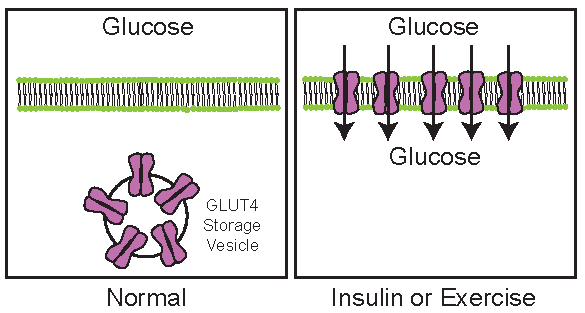
\includegraphics{figures/GLUT4-Trafficking.pdf}
\caption{Regulation of glucose uptake in muscle and adipocytes.  In these cells, glucose cannot enter unless insulin or AMPK stimulates the translocation of GLUT4 from intracellular GLUT4 storage vesicles to the plasma membrane.}
\label{fig:GLUT4-Trafficking}
\end{marginfigure}


GLUT4 on the other hand is the main transporter in muscle and adipocyte cells.  GLUT4 is normally present on intracellular vesicles within the cell and is therefore unable to conduct glucose into the cell.  When insulin is present, these vesicles fuse with the plasma membrane of these cells, placing GLUT4 transporters on the plasma membrane, and allowing for glucose to enter down its concentration gradient (see Figure \ref{fig:GLUT4-Trafficking}).  GLUT4 trafficking is the first regulated step for glucose oxidation and storage in muscle and fat cells.  For more details on how GLUT4 trafficking is regulated see \citet{Leto2013}.  GLUT4 translocation in muscle cells is also stimulated by exercise.  This is dependent on a protein kinase called AMPK, which is activated when AMP levels are high (or energy is low).  Improving glucose disposal rates, by allowing glucose into muscle is one major advantage of exercise in type 2 diabetics, who are resistant to the effects of insulin.  For more details on exercise-induced glucose uptake see \citet{Richter2013}.


\newthought{Glycolysis occurs in the cytoplasm of cells.}  All of glycolysis occurs in the cytoplasm of cells, unlike the TCA cycle or the electron transport chain, which require mitochondria.  As we will discuss later in the semester, mitochondria are also required for the oxidation of fatty acids and some amino acids.  This means that cells with few or no mitochondria (fast-twitch muscle fibers, or red blood cells for example) are highly dependent on glycolysis to generate ATP.

\subsection{The conversion of glucose to glucose-6-phosphate}

\newthought{There are two enzymes that catalyse the first step after glucose enters the cell.}   This step phosphorylates glucose at the 6 position, generating glucose-6-phosphate (G6P).  This is the first of two ATP consuming steps in glycolysis:

\begin{equation}\label{eq:glucokinase}
Glucose + ATP \rightarrow G6P
\end{equation}

In liver cells\sidenote{also known as hepatocytes.} and pancreas cells, this is done by an enzyme called \emph{glucokinase}.  This is a co-operative enzyme\sidenote{If you forgot what this means, review the metabolic control systems handout.} that has a very high maximal catalytic rate (V$_{max}$).  This means that at low levels of glucose, very little glucose is phosphorylated but at high levels of glucose, G6P can be produced at high rates. This is especially useful in the liver to prevent glucose oxidation in the liver when glucose levels are low indicating that glucose is needed for peripheral tissue use more urgently. Another way to think about this, is that the co-operativity of glucokinase means that its activity is dependent on glucose levels in the cell.  This means that glucokinase can serve as an intracellular glucose sensor.

\begin{marginfigure}
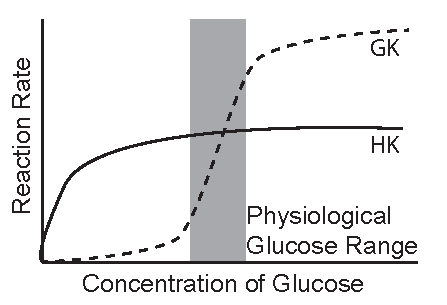
\includegraphics{figures/gk-hk-kinetics.pdf}
\caption{Schematic of the kinetics of glucokinase (GK) and hexokinase (HK).  Not the differences in K$_m$, V$_max$ and co-operativity between these enzymes.}
\label{fig:gk-hk-kinetics}
\end{marginfigure}

\newthought{Hexokinase is a high affinity enzyme} that catalyzes the same reaction in most other cells, for example muscle and adipose cells.  This means that it is very efficient even at low glucose concentrations, but does not have as high of a maximum rate\sidenote{It is important that you understand the differences in glucose affinity and V$_{max}$ between glucokinase and hexokinase and the consequences of these differences.}.  This is illustrated in Figure \ref{fig:gk-hk-kinetics}. This is especially useful in the muscles to ensure they oxidize glucose even at low glucose levels as the muscles always utilize energy. Hexokinase is regulated by negative feedback from its product G6P. Hence, an increase in G6P will downregulate the function of Hexokinase.  In contrast to hexokinase, there is no allosteric regulation of glucokinase.  Think about the differences in how glucose enters these cells, in contrast to liver cells and how the kinetics relate to the regulation of glucose uptake.  The differences between glucokinase and hexokinase are summarized in Table \ref{tab:glucokinase}.

\begin{table}
\centering
\caption{Differences between glucokinase and hexokinase.}
\label{tab:glucokinase}
\begin{tabular}{cccc}
\hline
\textbf {Enzyme} & \textbf{Kinetics}  & \textbf{Regulation}  & \textbf{Tissues}\\
\hline
Hexokinase & High Affinity & G6P (-) & Muscle/Adipose\\
Glucokinase & Co-operative & & Pancreas/Liver\\

\hline
\end{tabular}
\end{table}

\newthought{The reverse reaction of GK is the dephosphorylation of G6P to glucose, and primarily occurs in the liver.}  This is because most cells do not express Glucose-6-phosphatase (G6Pase), the enzyme that converts G6P back to glucose.  In the liver, G6Pase allows for dephosphorylated glucose to be released back into the blood, the last step in gluconeogenesis or hepatic glycogenolysis.\sidenote{Which will be discussed three lectures from now.}  This is relevant because in non-hepatic cells, the phosphorylation of glucose is \emph{irreversible} and traps glucose within the cell\sidenote{Think about why the co-operative properties of glucokinase work in tandem with the ability to dephosphorylate glucose in liver cells.}.

\subsection{What are the fates of glucose-6-phosphate?}

Phosphorylated glucose (G6P) can enter four separate pathways (3 in non-hepatic tissues), depending on the relative activities of the rate limiting steps in these pathways.  If glycogen synthase (GS) activity is elevated, glucose can become stored as glycogen.  If G6P Dehydrogenase (G6PDH) activity is elevated, glucose will flow through the pentose phosphate shunt (PPS).  Glycolysis will proceed if phosphofructokinase-1 (PFK1) is active.  These routes are summarized in Figure \ref{fig:g6p-fates}.

\begin{marginfigure}
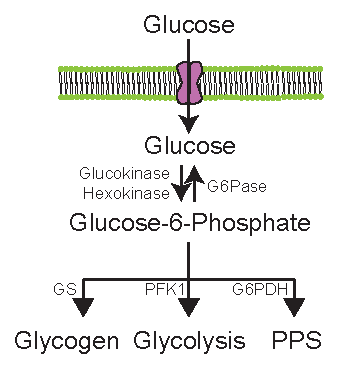
\includegraphics{figures/g6p-fates.pdf}
\caption{Fates of phosphorylated glucose and key rate limiting enzymes of each pathway.  Details of each pathway will be discussed in forthcoming lectures.}
\label{fig:g6p-fates}
\end{marginfigure}

\subsection{The first committed step of glycolysis is catalysed by PFK1}

The most important regulatory step that controls flow through glycolysis is catalyzed by PFK1\sidenote{For all these reactions G indicates Glucose, F indicates Fructose, GA indicates Glyceraldehyde and PG indicates Phosphoglycerate.}.  This is the second ATP consuming step, and the first committed step of glycolysis.  \sidenote{Reaction \ref{eq:pgm}, catalyzed by Phosphoglucose isomerase is a reversible, equilibrium reaction}:

\begin{equation}\label{eq:pgm}
G6P \rightleftharpoons F6P
\end{equation}

\begin{equation}\label{eq:pfk1}
F6P + ATP \rightarrow F16bP
\end{equation}

\begin{margintable}
\centering
\caption{Regulators of PFK1 activity}
\label{tab:pfk1-regulators}
\begin{tabular}{cc}
\hline
\textbf {Molecule} & \textbf{Direction}  \\
\hline
F2,6bP & Positive \\
AMP & Positive \\
ATP & Negative \\
Citrate & Negative \\
\hline
\end{tabular}
\end{margintable}

Because this is such an important regulatory node, there are several facets to the regulation of PFK1.  This is accomplished via four allosteric regulators, listed in Table \ref{tab:pfk1-regulators}.  Citrate is a part of the TCA cycle which we will discuss next lecture, and is also an indicator of sufficient fatty acids and acetyl-CoA (as we will discuss in the lipids unit).  Elevations in citrate indicate that there are sufficient molecules in the TCA cycle, a condition known as \emph{anaplerosis}\sidenote{Anaplerosis is a condition where the TCA cycle intermediates build up due to increased rate of metabolic reactions that feed into the TCA cycle.}.  Functionally, this means that when there are sufficient metabolites downstream of glycolysis, glycolysis is impaired at the PFK1 step.  This is known as negative feedback and is common in many of the pathways we will discuss this semester.

\newthought{ATP and AMP levels indicate the cellular energy status.}  In terms of PFK1 regulation, this means that when energy is low (low ATP/high AMP), PFK1 is activated and glycolysis (which is energy generating) proceeds.  On the other hand, when ATP levels are high and AMP levels are low (\textit{e.g.} in a liver cell after a meal), PFK1 can be inactivated and G6P will instead be stored as glycogen or enter the PPS.  This is one way in which energy can control glycolytic flux.

\begin{marginfigure}
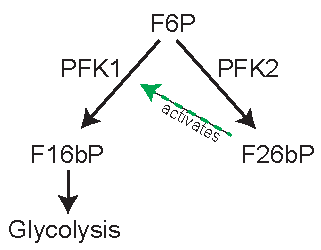
\includegraphics{figures/pfk1-pfk2-regulation.pdf}
\caption{Regulation of PFK1 by F26bP and PFK2.}
\label{fig:pfk1-pfk2-regulation}
\end{marginfigure}

\newthought{Fructose-2,6-bisphosphate is the most potent regulator of PFK1 activity.}  This molecule is generated from the same Fructose-6-phosphate (F6P) precursor that PFK1 acts on, but instead phosphorylates F6P on the 2-position.  This reaction is catalyzed by an enzyme known as PFK2.  This mechanism is known as feed-forward regulation, and means that when F6P builds up, it can be converted to F26bP, this in turn activates PFK1 to relieve the buildup of F6P in the cytoplasm\sidenote{An analogy for this might be if you are stuck in traffic and honk (to signal the traffic ahead to move faster).}.  The relationship between PFK1 and PFK2 is illustrated in Figure \ref{fig:pfk1-pfk2-regulation}.

\newthought{PFK2 is regulated by reversible phosphorylation in the liver.}  PFK2 activity is \emph{inhibited} by PKA-dependent phosphorylation \citep{VanSchaftingen1981}.  PKA in the liver is activated by hormones such as glucagon and epinephrine.  One biological goal of these hormones in the liver is to \emph{promote gluconeogensis}, and therefore it would be counterproductive to have glycolysis occuring at the same time.  As such, by reducing PFK2 activity (and reducing F26bP levels), PFK1 activity and glycolytic flux is all reduced.\sidenote{I appreciate that this is a lot of regulation, so I recommend sketching out PFK1/PFK2 and the various positive and negative regulators on your own.  Take a step back and think about what would cause these regulators to change, and how this would affect glycolytic flux.  Think about whether this would make "sense" based on what glycolysis is doing.}  As we will discuss a little later on, PKA-mediated inhibition of PFK2 does not occur in muscle cells.

\newthought{The next several steps of glycolysis are neither regulated nor rate limiting.}  In general, the F16bP molecule is broken in two by aldolase, then each part is rapidly converted into phosphoenolpyruvate via the following reactions:

\begin{equation}\label{eq:aldolase-a}
F16bP \rightleftharpoons DHAP+ GA3P
\end{equation}

\begin{equation}\label{eq:g3pdh}
GA3P + NAD+ \rightleftharpoons 1,3bPG  + NADH
\end{equation}

\begin{equation}\label{eq:pgk}
1,3bPG + ADP \rightleftharpoons 3PG + ATP
\end{equation}

\begin{equation}
3PG \rightleftharpoons 2PG
\end{equation}

\begin{equation}
2PG \rightleftharpoons Phosphoenolpyruvate
\end{equation}

Note that in reactions \ref{eq:g3pdh} and \ref{eq:pgk}, there is generation of NADH and ATP respectively\sidenote{Remember, since glucose was broken in two pieces in reaction \ref{eq:aldolase-a}, one glucose generates two ATP and two NADH at this step.}.  ATP is the primary fuel source in cells, and one molecule of NADH can be converted into 2.5 molecules of ATP via the electron transport chain\sidenote{Discussed next lecture.}.  

The second point, which we will come back to as it relates to lipid synthesis, is that the glycerol backbone, needed to generate triglycerides, can be derived from DHAP\sidenote{This is known as glyceroneogenesis.  Alternately, if glycerol levels are abundant, it can be recycled back into triglycerides.}.  This is important in the context of esterifying fatty acids into triglycerides, as three fatty acids require one activated glycerol backbone.  On the other hand, when glycerol is broken down, it becomes DHAP and enters the glycolytic pathway where it can be processed to pyruvate or converted to glucose.  Glycerol is a major gluconeogenic substrate, and again enters the glycolytic pathway as DHAP and then is converted back to glucose via mechanisms we will discuss in later lectures.

\subsection{Pyruvate kinase regulates conversion to pyruvate}

\begin{equation}\label{eq:pk}
PEP + ADP \rightarrow Pyruvate + ATP
\end{equation}

\begin{marginfigure}
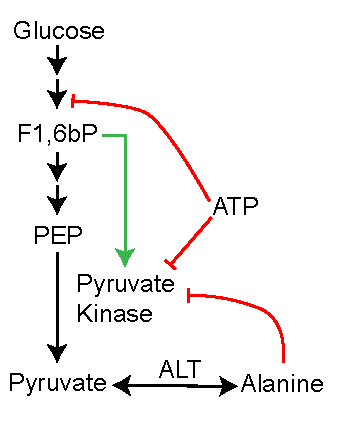
\includegraphics{figures/pk-regulation.pdf}
\caption{Regulation of pyruvate kinase in the liver.  In the muscle, neither ATP nor Alanine play important roles.  PKA indicates inhibitory phosphorylation of Pyruvate Kinase in response to glucagon or adrenaline.}
\label{fig:pk-regulation}
\end{marginfigure}

The last step of glycolysis catalyzes the \emph{irreversible} reaction of phosphoenolpyruvate (PEP) to pyruvate, and is catalysed by Pyruvate Kinase.  This is the last point of regulation in glycolysis.    Fructose-1,6-bisphosphate (F1,6bP) is the product of PFK1, and functions as a \emph{feed-forward} regulator of pyruvate kinase activity (see Figure \ref{fig:pk-regulation}).  ATP, similar to its inhibitory role on PFK1, reduces glycolytic flux when energy is not needed and thus inhibits Pyruvate Kinase function.  Alanine, on the other hand, is an amino acid that is easily interconverted with Pyruvate by the enzyme Alanine Aminotransferase (ALT)\sidenote{This will be discussed in the amino acid catabolism lecture.}.  As a marker for amino acid availability, Alanine reduces liver Pyruvate Kinase activity when there is less of a need to use glucose as fuel\sidenote{The muscle isoforms of Pyruvate Kinase is \emph{not} inhibited by ATP or Alanine, but is still subject to feed-forward regulation by F1,6bP.  The adipocyte isoform (PKM2) is also activated by Serine \citep{Christofk2008a} and is expressed in a variety of tumors.  It is an emerging anti-cancer target.}.  This is because the cell can use Alanine, rather than Phosphoenolpyruvate to generate Pyruvate.

\newthought{Similar to PFK2, Pyruvate kinase is inhibited by PKA-dependent protein phosphorylation.}  In the liver, glucagon or adrenaline can inhibit glycolysis at two steps, PFK2 (described above) and also at the Pyruvate Kinase step.  In both cases, this is important to prevent glycolysis and gluconeogenesis from occurring simultaneously.  Again, muscle cell Pyruvate Kinase is not inhibited in this manner.

\subsection{The fate of pyruvate}

Pyruvate can go in one of four directions in the cell, depending on the activity of Pyruvate Dehydrogenase (PDH) and the relative levels of Alanine in the cell.  The regulation of PDH is very important for aerobic respiration, and will be discussed next lecture.  These fates are described in Table \ref{tab:pyruvate-fates}.  In general, if Alanine is sufficient and PDH activity is low or absent, then pyruvate is converted to lactate via Lactate Dehydrogenase and released from the cell.  This is known as anaerobic respiration and is important for fast-twitch muscle fibers and in conditions where oxygen levels are low.  Pyruvate can also be easily converted to and from Alanine, via Alanine Aminotransferase (ALT)\sidenote{We will cover how the non-essential amino acids are synthesized later in this course.}.  Finally, as we will cover in the lectures on the TCA cycle, when acetyl-CoA levels are high\sidenote{Indicating reduced TCA/ETC flux, but sufficient acetyl-CoA production.  Think about under which conditions this might occur.}, Pyruvate can be converted to Oxaloacetate, a process known as anaplerosis.
\\[0.6cm]

\begin{table}
\centering
\caption{Potential fates of pyruvate.  While several of these enzymes and processes have not been covered yet, we will discuss all of these later in the semester.}
\label{tab:pyruvate-fates}
\begin{tabular}{ccc}
\hline
\textbf {Pyruvate Fate} & \textbf{Conditions}  & \textbf{Key Enzyme} \\
\hline
TCA cycle & High PDH Activity & Pyruvate Dehydrogenase \\
Lactate & Low PDH Activity & Lactate Dehydrogenase \\
Alanine & Low Ala, High Glu & Alanine Aminotransferase\\
Oxaloacetate & High Acetyl-CoA & Pyruvate Carboxylase \\
\hline
\end{tabular}
\end{table}

\section{Energy production by glycolysis}

Glycolysis occurs in three phases:

\begin{enumerate}
\item An investment phase, which uses two molecules of ATP (see reactions \ref{eq:glucokinase} and \ref{eq:pfk1}).  This "charges" the glucose molecule, providing it with enough energy to be split into two 3-carbon molecules.  \textbf{At this stage there is a net usage of two ATP molecules per molecule of glucose.}
\item The cleavage step, performed by aldolase A, immediately after the highly regulated PFK1 step (see reaction \ref{eq:aldolase-a}).  This is a very energetically costly step, as breaking a carbon-carbon bond is quite difficult\sidenote{The standard free energy of this step is +28 kcal/mol, making it highly endothermic.  For more details on how Fructose-1,6-bisphosphate buildup allows this difficult reaction to occur, see \url{http://sandwalk.blogspot.com/2007/10/aldolase-reaction-and-steady-state.html}}.  This cleavage means that one glucose molecule may eventually generate \textbf{two} Pyruvate molecules.
\item The catabolism of each molecule of glyceraldehyde-3-phosphate (GA3P) to pyruvate generates two molecules of ATP via substrate-level phosphorylation\sidenote{Substrate level phosphorylation is the production of ATP by direct transfer from another phosphorylated compound.} (see reactions \ref{eq:pgk} and \ref{eq:pk}).  There is also the reduction of one NAD+ molecule into NADH (see reaction \ref{eq:g3pdh}).  NADH, as we will discuss in the unit on the electron transport chain is equivalent to 2.5 ATP molecules.  Therefore this phase produces a total of 4.5 ATP molecules per GA3P, or \textbf{9 molecules per glucose molecule}.
\end{enumerate}

Glycolysis down to the level of pyruvate therefore uses up two ATP molecules, and generates the equivalent of 9 ATP molecules for a \textbf{net gain of 7 molecules of ATP per molecule of glucose.}  Full oxidation of glucose to CO\textsubscript{2} will eventually produce 32 molecules of ATP/glucose so at this stage there is quite a lot of energy remaining in pyruvate.

\subsection{Hormonal regulation of glycolysis}

\newthought{Insulin promotes glycolysis by several mechanisms.}  First, in muscle and adipose tissue, insulin promotes the translocation of GLUT4 to the plasma membrane, allowing for glucose entry into the cell.  This increases the levels of glucose, and glucose-6-phosphate in the cell.  Insulin also promotes the dephosphoryation of both PFK2 and Pyruvate Kinase in the liver \citep{PROBST1985}. Recall that in both cases, the dephosphorylated forms are \emph{more active}, so this increases the flux by which glucose gets converted to pyruvate or lactate.  The mechanisms by which insulin promotes these dephosphorylation events are still murky.

\newthought{Glycolysis is regulated differently in muscle than in liver tissues.}  There are splice variants\sidenote{Splice variants are different mRNA's which lead to different proteins, transcribed from the same gene.} of PFK2 that are expressed in a tissue specific manner.  In liver tissue the L-PFK2 isoform can be phosphorylated on Serine 32 resulting in its inhibition.  This residue is \emph{absent} in the muscle, brain and adipocyte isoforms.  Therefore, adrenaline/glucagon-mediated inhibition\sidenote{Via PKA-dependent phosphorylation.} and insulin-mediated activation (via dephosphorylation) is \emph{only} relevant for the liver isoform of PFK2.  The muscle and adipocyte PFK2 isoforms are not regulated by these hormones.  This means that glucagon or adrenaline will prevent glycolysis in liver cells but that adrenaline or glucagon will not prevent glycolysis in muscle cells\sidenote{There is a physiological advantage to this.   Think about what the consequence would be if adrenaline \emph{prevented} glycolysis in muscle cells, and why it would be advantageous to do this in liver cells.}.  Similarly, Pyruvate Kinase is inhibited by PKA, ATP and Alanine, only in the liver, but all Pyruvate Kinase isoforms are regulated positively by F16bP.  This means that the negative feedback of Pyruvate kinase by PKA, Alanine and ATP is not a factor in the regulation of adipocyte or muscle glycolysis.  

\newthought{Another level of control of glycolysis is transcriptional.}  There are certain conditions where it is helpful to increase glycolysis in a chronic and less rapidly reversible manner.  This is typically mediated by transcription factors which synthesize new glycolytic proteins, increasing the capacity by which glycolysis can occur.  There are several examples of this such as:

\begin{itemize}
\item Hypoxia, or reduced oxygen, via the transcription factor HIF\sidenote{Think about why glycolysis may be advantageous during oxygen deprivation.}.
\item Chronically elevated glucose levels (via the transcription factor ChREBP).    
\item Chronic glucagon stimulation (via the transcription factor CREB).
\end{itemize}

These transcriptional changes often affect the expression of the enzymes Pyruvate Kinase, Glucokinase and PFK2 \citep{Semenza1994,Kawaguchi2001}.  These changes are slower and more energetically costly than allosteric or post-translational changes.  As such, they are both longer lasting and harder to undo.

\section{Fructose metabolism}

Fructose, the other monosaccharide unit in sucrose is largely metabolized within the liver and intestine\sidenote{Intestinal fructose metabolism was recently explored in a recent paper by \citet{Jang2018}.  There is an \emph{optional} group project on GradeCraft that considers this work.  If you (and a couple other classmates) are interested in intestinal metabolism, give that a look.}  , compared to glucose which is metabolized in multiple tissues.  Within the liver, fructose enters the hepatocyte via facilitative GLUT5 channels, which are constitutively present on the plasma membrane. In terms of metabolism, fructose undergoes the following steps, catalyzed by ketohexokinase (reaction \ref{eq:ketohexokinase})\sidenote{also known as fructokinase}, aldolase B (reaction \ref{eq:aldolase}) then triose kinase (reaction \ref{eq:triose-kinase})\sidenote{Be careful here, fructose becomes F16bP then DHAP/G3P whereas glucose becomes F6P then F16bP then DHAP/GA3P.  These routes can be easily confused.}\sidenote{As an exercise, draw out the pathways by which glucose and fructose become pyruvate, calculate whether the ATP production is similar for these two monosaccharides.}.

\begin{equation}\label{eq:ketohexokinase}
Fructose + ATP \rightarrow Fructose-1-phosphate
\end{equation}

\begin{equation}\label{eq:aldolase}
Fructose-1-phosphate \rightleftharpoons Glyceraldehyde + DHAP
\end{equation}

\begin{equation}\label{eq:triose-kinase}
Glyceraldehyde + ATP \rightarrow GA3P
\end{equation}


\subsection{Fructose catabolism is independent of PFK1}

The products (DHAP and Glyceraldehyde-3-phosphate) are the same metabolites that are produced by the glycolytic step in reaction \ref{eq:aldolase-a}.  Importantly this step occurs \emph{after} the two key glycolytic regulatory steps at PFK1 and Glucokinase. Hence fructose feeds into the glycolytic flux past the two regulatory points of PFK1 and Glucokinase. This has very important ramifications for how fructolysis\sidenote{The breakdown of fructose into pyruvate/lactate.} is regulated  relative to glycolysis.  Since the regulatory steps that can normally control the flow of glucose are uncontrolled for fructose, fructose is converted rapidly to its end-products, whether there is energy demand or not.  This is biochemical basis by which fructose is thought to be more prone to become acetyl-CoA and then fatty acids\sidenote{Think about how citrate can control glucose but not fructose breakdown.}.  Similarly, as we will discuss for unit on gluconeogenesis, fructose can very easily be converted to glucose with little regulatory oversight \citep{Kim2016d}.

\subsection{Fructose consumption has been linked to both obesity and liver disease}

Fructose is normally present at high levels in fruit, or as the disaccharide sucrose, which has a 1:1 ratio of glucose:fructose.  For ease of handling and production, high fructose corn syrup (HFCS) has been in widespread use since the 1970s, particularly in sugar-sweetened beverages.  HFCS generally contains 45-60\% fructose with the remaining as glucose.   While as recently as 2014, the Food and Drug Administration has declared HFCS safe as a food ingredient, epidemiological studies suggested HFCS may be associated with both obesity, and non-alcoholic fatty liver disease\sidenote{A liver disease that starts with lipid accumulation and inflammation of the liver, which can result in impaired liver function or eventually cirrhosis or some liver cancers.}.  A recent meta-analysis in this area was inconclusive, as it was difficult to separate the effects of added calories due to HFCS from direct metabolic effects of this sweetener \citep{Chung2014}.

\subsection{Disorders of fructose metabolism}

There are two inborn errors of fructose metabolism, defects in either Fructokinase or Aldolase B\sidenote{This is a different enzyme from Aldolase A, which is part of glycolysis and shown in reaction \ref{eq:aldolase}.}.  In the case of individuals with Fructokinase deficiency, this is generally not pathological, since Fructose is not phosphorylated, and therefore is not trapped in cells.  Patients with Fructokinase deficiency have very high circulating levels of Fructose in their blood, but are otherwise normal.  On the other hand, Aldolase B deficiency means that Fructose becomes trapped at the Fructose-1-phosphate step \citep{Cross1988}\sidenote{If you want to explore mutations in any of the enzymes we discuss in more detail, I suggest going to the website \url{http://bravo.sph.umich.edu}, enter the gene name, scroll down, click on LOF (loss of function) then click on any of the variants to see their incidence in various populations.  The gene name for Aldolase B for example is \textit{ALDOB}.}.  This occurs in approximately 1 in 20,000 to 30,000 individuals.  This intermediary metabolite builds up, wasting ATP and resulting in liver cirrhosis, hypoglycemia and kidney damage\sidenote{Think about, from a dietary perspective how this disease could be managed.}.

\section{Galactose metabolism}

Galactose, the other monosaccharide in lactose is taken up in the liver via GLUT2.  In contrast to Fructose, Galactose enters glycolysis near the early steps of glycolysis and is subject to similar regulatory steps.  The initial steps of galactolysis are catalyzed by the enzymes galactokinase and GALT\sidenote{Galactose-1-phosphate uridylyltransferase, shown in reaction \ref{eq:galt}.  This is \emph{not} the same thing as Gut-Associated Lymphoid Tissue, which is also abbreviated as GALT and was discussed as it relates to the digestive system.} or phosphoglucomutase and result in the production of Glucose-6-phosphate:

\begin{equation}
Galactose + ATP \rightarrow Gal1P
\end{equation}

\begin{equation} \label{eq:galt}
Gal1P + UDP-Glucose \rightleftharpoons G1P + UDP-Gal
\end{equation}

\begin{equation}
G1P \rightleftharpoons G6P
\end{equation}

Glucose-6-phosphate then proceeds as normal, becoming dephosphorylated to glucose, or processed through glycolysis, glycogenesis or the pentose phosphate pathway (see Figure \ref{fig:g6p-fates}).  The UDP-galactose generated in reaction \ref{eq:galt} is regenerated back to UDP glucose by another enzyme called UDP-Galactose Epimerase, which catalyzes this reaction:

\begin{equation}
UDP-Galactose \rightleftharpoons UDP-Glucose
\end{equation}

Inborn errors of GALT or UDP-Galactose epimerase lead to galactose intolerance and a buildup of Galactose-1-phosphate in tissues and the blood.

\bibliography{library}
\bibliographystyle{plainnat}

\end{document}
